\documentclass[12pt,a4paper]{article}

% --- Encodage et langue ---
\usepackage[utf8]{inputenc}
\usepackage[T1]{fontenc}
\usepackage{lmodern}

% --- Maths ---
\usepackage{amsmath,amssymb,amsthm}

% --- Mise en page ---
\usepackage[top=2.5cm,bottom=2.5cm,left=2.8cm,right=2.8cm]{geometry}
\usepackage{parskip}

% --- Tableaux ---
\usepackage{booktabs}
\usepackage{array}
\usepackage{multirow}

% --- Figures et couleurs ---
\usepackage{tikz}
\usetikzlibrary{arrows.meta, positioning, decorations.pathreplacing, calc, fit, backgrounds}
\usepackage{xcolor}
\usepackage{pgfplots}
\pgfplotsset{compat=1.18}
\usepgfplotslibrary{fillbetween}

% --- Liens ---
\usepackage{hyperref}
\hypersetup{colorlinks=true, linkcolor=blue!60!black, citecolor=blue!60!black}

% --- Macros (cohérentes avec convergence_sans_bruit.tex) ---
\newcommand{\Inc}{\ensuremath{\mathrm{Include}}}
\newcommand{\Exc}{\ensuremath{\mathrm{Exclude}}}
\newcommand{\vbar}{\bar{v}}
\newcommand{\code}[1]{\texttt{#1}}

% --- Environnement pour les notes/encadrés ---
\theoremstyle{remark}
\newtheorem{note}{Note}[section]
\newtheorem{exemple}{Exemple fil rouge}[section]

% ======================================================
\begin{document}
% ======================================================

\begin{center}
  {\LARGE\bfseries Anatomie du moteur}\\[6pt]
  {\large Du dataset à la sortie d'une clause, puis à un round de boosting}\\[4pt]
  {\large\itshape Un seul algorithme, appliqué identiquement à Iris, Digits, XOR et MNIST}
\end{center}

\vspace{1em}
\hrule
\vspace{1.2em}

\begin{figure}[h]
\centering
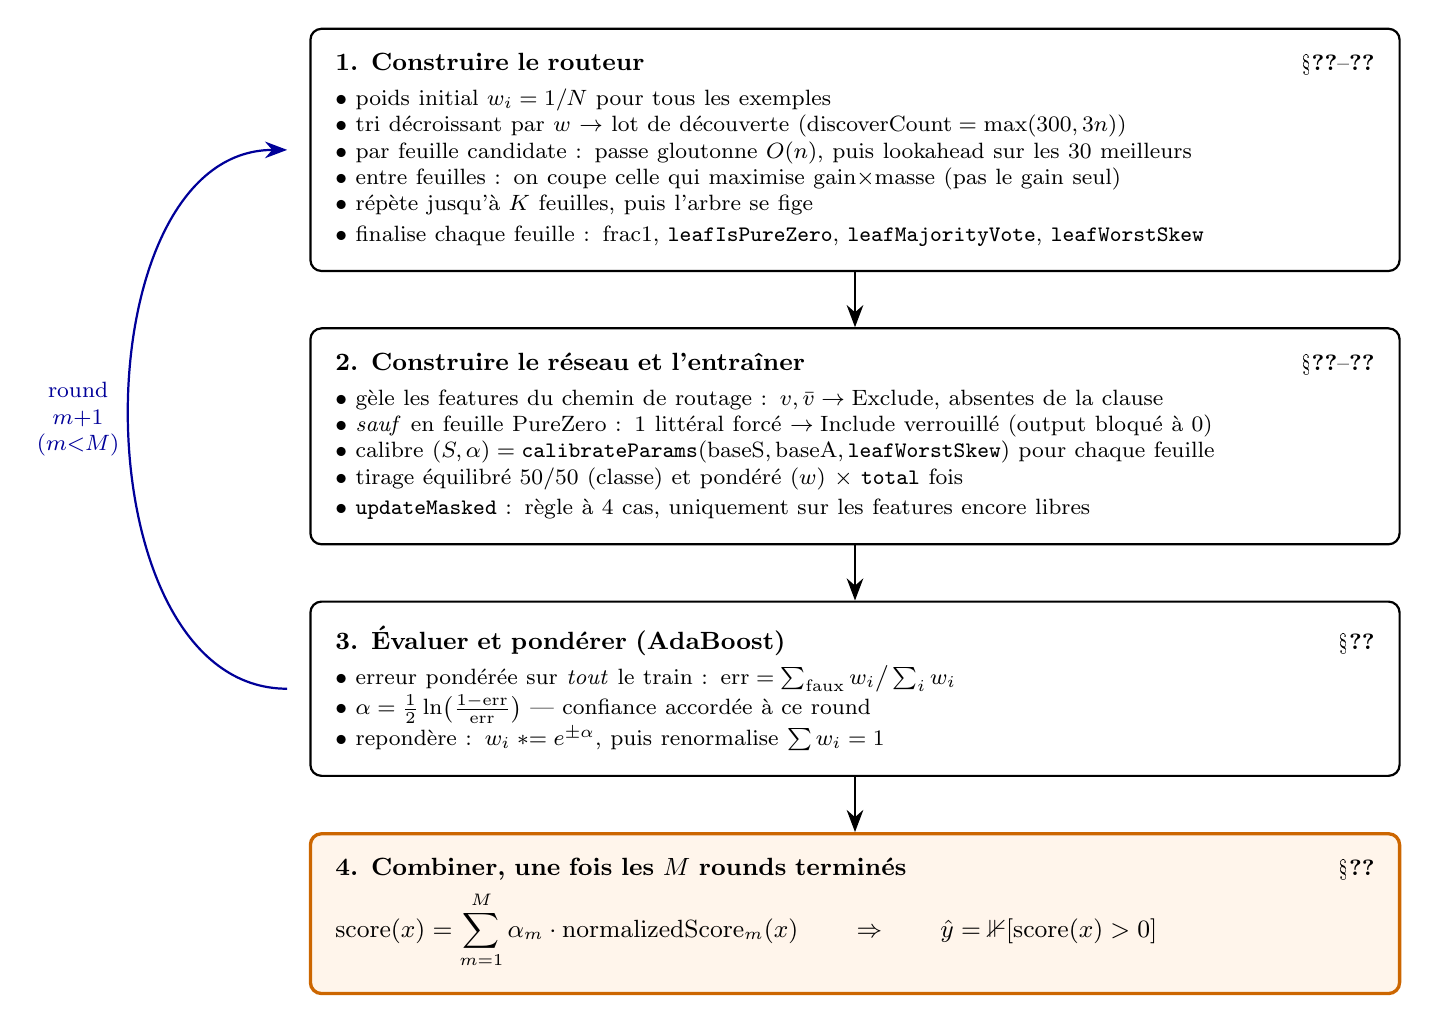
\begin{tikzpicture}[
  bigbox/.style={draw, thick, rounded corners, align=left, font=\small, text width=13.2cm, inner sep=9pt},
  finalbox/.style={draw=orange!80!black, very thick, rounded corners, align=left, font=\small,
                    fill=orange!8, text width=13.2cm, inner sep=9pt},
  arr/.style={-{Stealth[length=8pt]}, thick},
  node distance=0.7cm
]
\node[bigbox] (b1) {\textbf{1. Construire le routeur} \hfill{\footnotesize\S\ref{sec:router}--\ref{sec:leaves}}\\[3pt]
\footnotesize
$\bullet$ poids initial $w_i=1/N$ pour tous les exemples\\
$\bullet$ tri décroissant par $w$ $\to$ lot de découverte ($\mathrm{discoverCount}=\max(300,3n)$)\\
$\bullet$ par feuille candidate : passe gloutonne $O(n)$, puis lookahead sur les 30 meilleurs\\
$\bullet$ entre feuilles : on coupe celle qui maximise gain$\times$masse (pas le gain seul)\\
$\bullet$ répète jusqu'à $K$ feuilles, puis l'arbre se fige\\
$\bullet$ finalise chaque feuille : frac1, \code{leafIsPureZero}, \code{leafMajorityVote}, \code{leafWorstSkew}};

\node[bigbox, below=of b1] (b2) {\textbf{2. Construire le réseau et l'entraîner} \hfill{\footnotesize\S\ref{sec:calib}--\ref{sec:update}}\\[3pt]
\footnotesize
$\bullet$ gèle les features du chemin de routage : $v,\vbar\to\Exc$, absentes de la clause\\
$\bullet$ \emph{sauf} en feuille PureZero : 1 littéral forcé $\to\Inc$ verrouillé (output bloqué à 0)\\
$\bullet$ calibre $(S,\alpha)=\code{calibrateParams}(\mathrm{baseS},\mathrm{baseA},\code{leafWorstSkew})$ pour chaque feuille\\
$\bullet$ tirage équilibré 50/50 (classe) et pondéré ($w$) $\times$ \code{total} fois\\
$\bullet$ \code{updateMasked} : règle à 4 cas, uniquement sur les features encore libres};

\node[bigbox, below=of b2] (b3) {\textbf{3. Évaluer et pondérer (AdaBoost)} \hfill{\footnotesize\S\ref{sec:combine}}\\[3pt]
\footnotesize
$\bullet$ erreur pondérée sur \emph{tout} le train : $\mathrm{err}=\sum_{\text{faux}} w_i \big/ \sum_i w_i$\\
$\bullet$ $\alpha=\tfrac12\ln\!\big(\tfrac{1-\mathrm{err}}{\mathrm{err}}\big)$ --- confiance accordée à ce round\\
$\bullet$ repondère : $w_i\mathrel{*}=e^{\pm\alpha}$, puis renormalise $\sum w_i=1$};

\node[finalbox, below=of b3] (b4) {\textbf{4. Combiner, une fois les $M$ rounds terminés} \hfill{\footnotesize\S\ref{sec:combine}}\\[3pt]
$\mathrm{score}(x)=\displaystyle\sum_{m=1}^{M}\alpha_m\cdot\mathrm{normalizedScore}_m(x)
\qquad\Rightarrow\qquad \hat y = \mathbb{1}[\mathrm{score}(x)>0]$};

\draw[arr] (b1) -- (b2);
\draw[arr] (b2) -- (b3);
\draw[arr] (b3) -- (b4);
\draw[arr, blue!60!black] ([xshift=-8pt]b3.west) to[out=180,in=180]
  node[left,font=\footnotesize,text=blue!60!black,align=center]{round\\$m{+}1$\\($m{<}M$)} ([xshift=-8pt]b1.west);
\end{tikzpicture}
\caption{Vue d'ensemble complète du mécanisme, tous les niveaux inclus :
construction du routeur (deux passes + sélection par masse), construction et
calibration du réseau, entraînement, évaluation/repondération AdaBoost, et
combinaison finale des $M$ réseaux. Chaque puce renvoie à la section qui la
détaille avec l'exemple fil rouge chiffré.}
\label{fig:master-overview}
\end{figure}

\clearpage
\tableofcontents

\newpage

% ======================================================
\section{L'exemple fil rouge}
% ======================================================

Pour rendre chaque étape concrète, on utilise partout dans ce document le même
petit dataset jouet : $n=4$ features booléennes $x=(x_0,x_1,x_2,x_3)$, une
étiquette $y\in\{0,1\}$, et un routeur déjà construit à $K=3$ feuilles par deux
coupures successives :

\begin{itemize}
  \item la racine coupe sur $x_0$ : à gauche ($x_0{=}0$) $\to$ \textbf{feuille A} ;
  \item à droite ($x_0{=}1$), une deuxième coupure sur $x_2$ donne
        \textbf{feuille B} ($x_2{=}0$) et \textbf{feuille C} ($x_2{=}1$).
\end{itemize}

\begin{figure}[h]
\centering
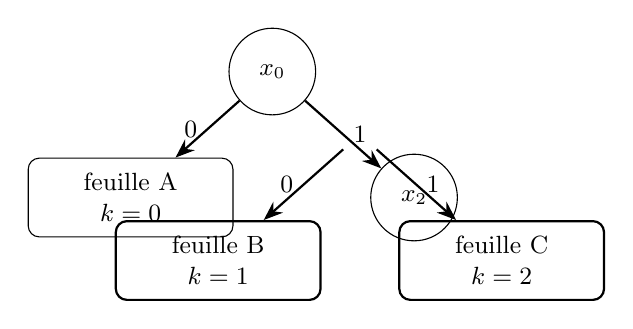
\begin{tikzpicture}[
  node/.style={draw, circle, minimum size=1.1cm, font=\small},
  leaf/.style={draw, rounded corners, minimum width=2.6cm, minimum height=1cm, font=\small, align=center},
  level distance=1.6cm,
  sibling distance=3.6cm,
  edge from parent/.style={draw, thick, -{Stealth[length=7pt]}}
]
\node[node] (root) {$x_0$}
  child { node[leaf] (A) {feuille A\\$k=0$} edge from parent node[left,font=\small] {$0$} }
  child { node[node] (x2) {$x_2$} edge from parent node[right,font=\small] {$1$}
    child { node[leaf] (B) {feuille B\\$k=1$} edge from parent node[left,font=\small] {$0$} }
    child { node[leaf] (C) {feuille C\\$k=2$} edge from parent node[right,font=\small] {$1$} }
  };
\end{tikzpicture}
\caption{Le routeur jouet utilisé dans tout ce document : 2 coupures, 3 feuilles.
Feuille A : $x_0{=}0$ fixé (1 feature gelée). Feuille B et C : $x_0{=}1,x_2{\in}\{0,1\}$
fixés (2 features gelées), $x_1,x_3$ restent libres.}
\label{fig:toy-tree}
\end{figure}

Trois faits, calculés une fois pour toutes sur les exemples d'entraînement tombés
dans chaque feuille, complètent ce routeur (section~\ref{sec:leaves} pour le détail) :

\begin{center}
\renewcommand{\arraystretch}{1.25}
\begin{tabular}{lccc}
\toprule
 & \textbf{feuille A} ($k{=}0$) & \textbf{feuille B} ($k{=}1$) & \textbf{feuille C} ($k{=}2$) \\
\midrule
features gelées & $\{0\}$, fixée à $0$ & $\{0,2\}$, fixées à $(1,0)$ & $\{0,2\}$, fixées à $(1,1)$ \\
frac1 pondérée  & $0.03$ & $0.52$ & $0.18$ \\
\code{leafIsPureZero} & \textbf{vrai} & faux & faux \\
\bottomrule
\end{tabular}
\end{center}

\noindent La feuille A est donc \emph{presque toujours négative} (PureZero) --- on
y reviendra en détail à la section~\ref{sec:gel}.

% ======================================================
\section{Vue d'ensemble : le trajet d'un exemple, du dataset à la sortie}
% ======================================================

Avant de détailler la construction, voici tout le trajet d'un exemple à travers
un réseau \emph{déjà construit} --- ce que fait \code{MultiClauseNetwork::output(x)}.
Un réseau, c'est : un routeur figé (section~\ref{sec:router}) qui aiguille chaque
exemple vers l'une des $K$ clauses, et $K$ clauses, chacune un simple \textbf{ET
logique} de littéraux dont les automates ont été appris (section~\ref{sec:update}).

\begin{exemple}
On prend $x=(1,1,1,0)$. Le routeur teste $x_0{=}1$ (va à droite), puis $x_2{=}1$
(va à droite) : $x$ atterrit en \textbf{feuille C} ($k{=}2$). Supposons que la
clause de cette feuille ait appris, sur ses deux features libres $\{1,3\}$ :
$v[1]=\Inc$ (le littéral ``$x_1$'') et $\vbar[3]=\Inc$ (le littéral ``$\neg x_3$''),
tout le reste exclu.
\end{exemple}

\begin{figure}[h]
\centering
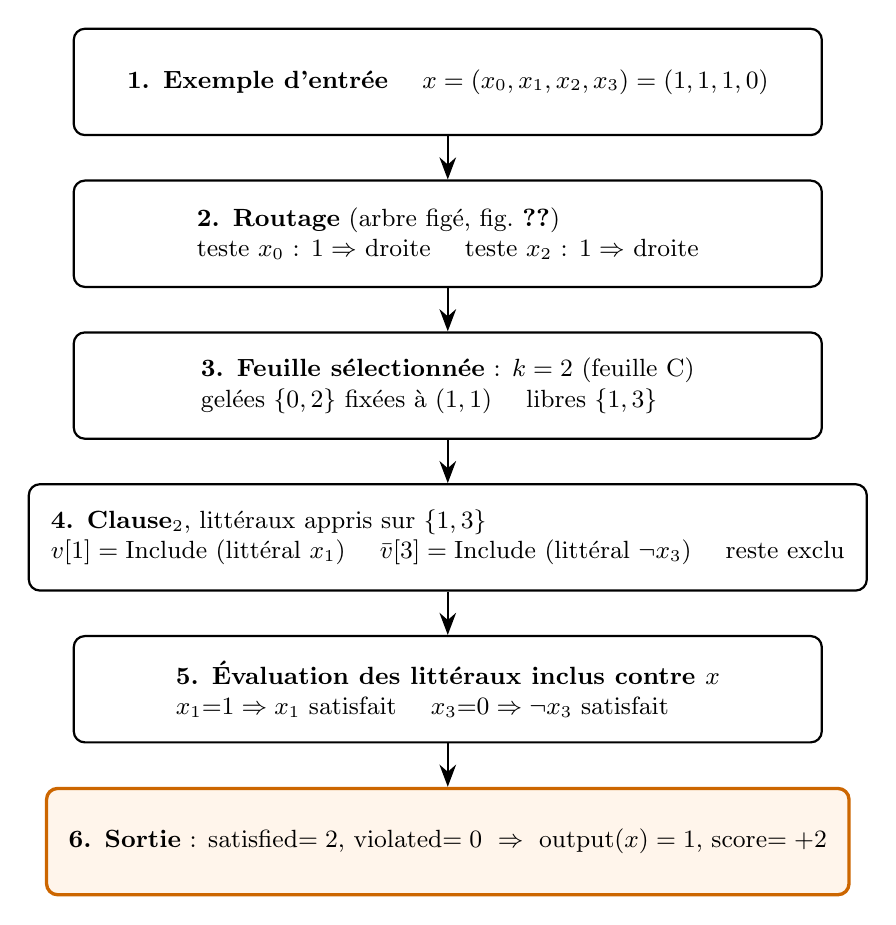
\begin{tikzpicture}[
  stage/.style={draw, rounded corners, thick, minimum width=9.5cm, minimum height=1.35cm,
                align=left, font=\small, inner sep=8pt},
  final/.style={stage, draw=orange!80!black, very thick, fill=orange!8, align=center},
  arr/.style={-{Stealth[length=8pt]}, thick},
  node distance=0.55cm
]
\node[stage, align=center] (s1) {\textbf{1. Exemple d'entrée} $\quad x=(x_0,x_1,x_2,x_3)=(1,1,1,0)$};
\node[stage, below=of s1] (s2) {\textbf{2. Routage} (arbre figé, fig.~\ref{fig:toy-tree})\\
  teste $x_0$ : $1\Rightarrow$ droite \quad teste $x_2$ : $1\Rightarrow$ droite};
\node[stage, below=of s2] (s3) {\textbf{3. Feuille sélectionnée} : $k=2$ (feuille C)\\
  gelées $\{0,2\}$ fixées à $(1,1)$ \quad libres $\{1,3\}$};
\node[stage, below=of s3] (s4) {\textbf{4. Clause$_2$}, littéraux appris sur $\{1,3\}$\\
  $v[1]=\Inc$ (littéral $x_1$) \quad $\vbar[3]=\Inc$ (littéral $\neg x_3$) \quad reste exclu};
\node[stage, below=of s4] (s5) {\textbf{5. Évaluation des littéraux inclus contre $x$}\\
  $x_1{=}1\Rightarrow x_1$ satisfait \quad $x_3{=}0\Rightarrow \neg x_3$ satisfait};
\node[final, below=of s5] (s6) {\textbf{6. Sortie} : satisfied$=2$, violated$=0$
  $\;\Rightarrow\;$ output$(x)=1$, score$=+2$};

\draw[arr] (s1) -- (s2);
\draw[arr] (s2) -- (s3);
\draw[arr] (s3) -- (s4);
\draw[arr] (s4) -- (s5);
\draw[arr] (s5) -- (s6);
\end{tikzpicture}
\caption{Le trajet complet d'un exemple, du dataset à la sortie d'une clause.
Chaque étape est développée dans une section dédiée : le routage
(sections~\ref{sec:router}--\ref{sec:leaves}), le gel des features
(section~\ref{sec:gel}), et l'évaluation/l'apprentissage de la clause
(section~\ref{sec:update}).}
\label{fig:pipeline-inference}
\end{figure}

\subsection{Rappel : que veut dire ``littéral inclus'' ?}

Chaque feature $i$ possède deux automates : $v[i]$ (associé au littéral $x_i$) et
$\vbar[i]$ (associé au littéral $\neg x_i$). Chacun a un état entier dans
$\{1,\dots,2N\}$ : au-dessus de $N$, le littéral est \Inc{} (il compte dans la
clause) ; à $N$ ou en-dessous, il est \Exc{} (il est ignoré). La clause est le ET
logique de tous les littéraux inclus. Elle est \textbf{violée} dès qu'un seul
littéral inclus est faux pour $x$ ; elle est \textbf{satisfaite} seulement si
\emph{tous} ses littéraux inclus sont vrais pour $x$ (ou si elle n'en a aucun).

\begin{figure}[h]
\centering
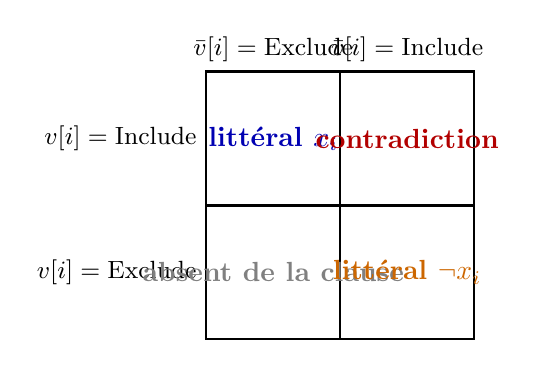
\begin{tikzpicture}[scale=0.85]
  \draw[thick] (0,0) rectangle (4,4);
  \draw[thick] (2,0) -- (2,4);
  \draw[thick] (0,2) -- (4,2);
  \node[above] at (1,4) {\small $\vbar[i] = \Exc$};
  \node[above] at (3,4) {\small $\vbar[i] = \Inc$};
  \node[left]  at (0,3) {\small $v[i] = \Inc$};
  \node[left]  at (0,1) {\small $v[i] = \Exc$};
  \node[font=\bfseries, text=blue!70!black] at (1,3) {littéral $x_i$};
  \node[font=\bfseries, text=red!70!black]  at (3,3) {contradiction};
  \node[font=\bfseries, text=gray]          at (1,1) {absent de la clause};
  \node[font=\bfseries, text=orange!80!black] at (3,1) {littéral $\neg x_i$};
\end{tikzpicture}
\caption{Les quatre configurations possibles de $(v[i],\vbar[i])$ pour une seule
feature $i$ (notation identique à \emph{convergence\_sans\_bruit.tex}). Le cas
``absent de la clause'' ($v,\vbar$ tous deux \Exc) est celui utilisé pour toute
feature gelée par le routeur (section~\ref{sec:gel}).}
\label{fig:config-rappel}
\end{figure}

% ======================================================
\section{Construire le routeur}\label{sec:router}
% ======================================================

Le routeur est construit \emph{une fois par round de boosting} par
\code{buildWeightedRouterTree}, sur un lot pondéré d'exemples. Son rôle : couper
l'espace des exemples en $K$ groupes (les feuilles), aussi purs que possible
vis-à-vis de $y$, en ajoutant une coupure à la fois.

\subsection{L'impureté de Gini pondérée}

Pour juger si une coupure est bonne, on mesure l'impureté de Gini \emph{pondérée}
d'un ensemble d'exemples $E$ :
\[
  \mathrm{wSum} = \sum_{e\in E} w_e, \qquad
  \mathrm{wPos} = \sum_{e\in E,\, y_e=1} w_e, \qquad
  p_1 = \frac{\mathrm{wPos}}{\mathrm{wSum}}, \qquad
  \mathrm{Gini}(E) = 2\,p_1(1-p_1).
\]
$\mathrm{Gini}(E)=0$ si $E$ est pur (tous $y_e$ identiques), $\mathrm{Gini}(E)=0.5$
si $E$ est parfaitement mélangé (50/50). Couper $E$ en $E_L,E_R$ sur une feature
$f$ donne un \textbf{gain} :
\[
  \mathrm{gain}(f) = \mathrm{Gini}(E) - \underbrace{\left[\frac{\mathrm{wSum}(E_L)}{\mathrm{wSum}(E)}\mathrm{Gini}(E_L)
  + \frac{\mathrm{wSum}(E_R)}{\mathrm{wSum}(E)}\mathrm{Gini}(E_R)\right]}_{\text{impureté pondérée après coupure}}.
\]

\subsection{L'algorithme, une feuille à la fois}

L'arbre part d'une seule feuille (la racine, qui contient tous les exemples du
lot). Tant qu'il y a moins de $K$ feuilles :

\begin{enumerate}
  \item pour \textbf{chaque feuille actuelle}, on cherche sa meilleure coupure
        possible (feature + gain), avec la méthode en 2 passes ci-dessous ;
  \item parmi toutes les feuilles, on choisit celle dont la coupure a le plus
        grand \textbf{gain $\times$ masse de la feuille} (section~\ref{sec:leafmass}) ;
  \item on coupe cette feuille en deux nouvelles feuilles, on retire l'ancienne,
        et on recommence.
\end{enumerate}

\begin{figure}[h]
\centering
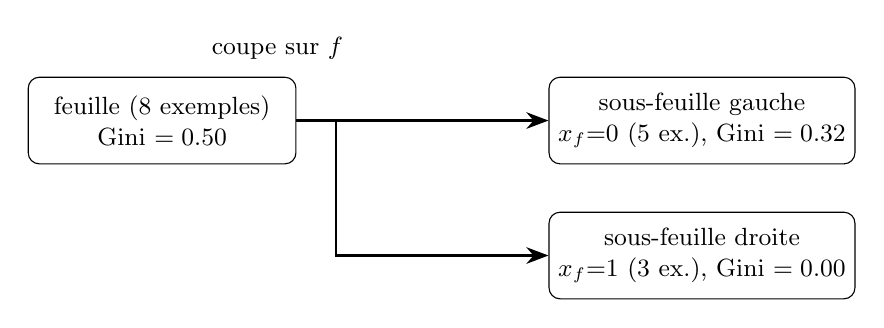
\begin{tikzpicture}[
  leaf/.style={draw, rounded corners, minimum width=3.4cm, minimum height=1.1cm, align=center, font=\small},
  arr/.style={-{Stealth[length=8pt]}, thick}
]
\node[leaf] (before) {feuille (8 exemples)\\Gini $=0.50$};
\node[leaf, right=3.2cm of before] (left)  {sous-feuille gauche\\$x_f{=}0$ (5 ex.), Gini $=0.32$};
\node[leaf, below=0.6cm of left] (right) {sous-feuille droite\\$x_f{=}1$ (3 ex.), Gini $=0.00$};
\draw[arr] (before.east) -- ++(0.5,0) |- (left.west);
\draw[arr] (before.east) -- ++(0.5,0) |- (right.west);
\node[font=\small, above right=0.1cm and -1.2cm of before] {coupe sur $f$};
\end{tikzpicture}
\caption{Une itération, en substance : une feuille se coupe en deux sur la
feature choisie. Le gain de cette coupure précise
serait ici $0.50 - (\tfrac58{\cdot}0.32+\tfrac38{\cdot}0.00)=0.30$. (Valeurs illustratives.)}
\label{fig:one-split}
\end{figure}

\subsection{Pourquoi deux passes : glouton, puis lookahead limité}

Une passe purement gloutonne (tester chaque feature seule, garder la meilleure)
suffit dans la grande majorité des cas, mais échoue sur des structures type XOR.
Exemple minimal à 2 features signal $x_0,x_1$ avec $y = x_0 \oplus x_1$ :

\begin{center}
\begin{tabular}{ccc}
\toprule
$x_0$ & $x_1$ & $y$ \\
\midrule
0 & 0 & 0 \\
0 & 1 & 1 \\
1 & 0 & 1 \\
1 & 1 & 0 \\
\bottomrule
\end{tabular}
\end{center}

\noindent Couper sur $x_0$ seul donne deux enfants à 50/50 ($x_0{=}0$ contient
$y{\in}\{0,1\}$ à parts égales, pareil pour $x_0{=}1$) : \textbf{gain nul}. Même
chose pour $x_1$ seul. Le signal n'existe que dans la \emph{combinaison} des deux
features --- une passe gloutonne ne voit donc, à tort, aucune raison de couper ici.

Le \textbf{lookahead} corrige ce problème : pour un candidat $f$, on simule un
\emph{deuxième} niveau de coupure sur chaque enfant (avec la meilleure feature
restante), et on mesure le gain à deux coups d'avance plutôt qu'à un seul. Sur
l'exemple ci-dessus, couper sur $x_0$ puis, dans chaque enfant, sur $x_1$, sépare
parfaitement $y$ --- le lookahead voit ce gain, la passe gloutonne ne le voit pas.

Le problème : simuler le lookahead sur les $n$ features coûterait $O(n^2)$,
intraitable pour MNIST ($n=784$). La solution retenue, \textbf{identique pour
tous les datasets} : classer d'abord toutes les features par gain glouton
($O(n)$), puis ne raffiner par lookahead que les \code{LOOKAHEAD\_TOPM = 30}
meilleures ($O(30\cdot n)$). Pour Iris ($n{=}16$) et XOR ($n{=}12$), $n<30$ donc
\emph{toutes} les features sont raffinées --- le comportement est celui du
lookahead complet. Pour Digits ($n{=}192$) et MNIST ($n{=}784$), seules les 30
meilleures le sont, ce qui suffit en pratique.

\begin{figure}[h]
\centering
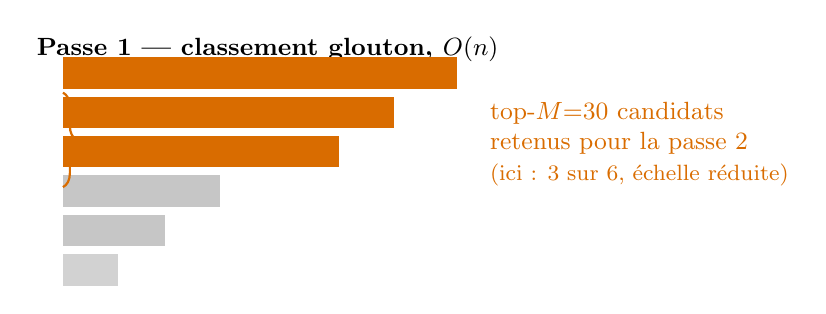
\begin{tikzpicture}
\node[font=\small\bfseries] at (2.6,3.6) {Passe 1 --- classement glouton, $O(n)$};
\foreach \i/\w/\c in {0/5.0/orange!85!black, 1/4.2/orange!85!black, 2/3.5/orange!85!black,
                      3/2.0/gray!45, 4/1.3/gray!45, 5/0.7/gray!35}{
  \pgfmathsetmacro{\y}{3.1-0.5*\i}
  \draw[fill=\c, draw=none] (0,\y) rectangle (\w,\y+0.4);
}
\draw[decorate, decoration={brace, amplitude=5pt}, thick, orange!85!black] (0,3.05) -- (0,1.85);
\node[font=\small, orange!85!black, right, align=left] at (5.3,2.4)
  {top-$M{=}30$ candidats\\retenus pour la passe 2\\\footnotesize(ici : 3 sur 6, échelle réduite)};
\end{tikzpicture}

\vspace{0.5em}

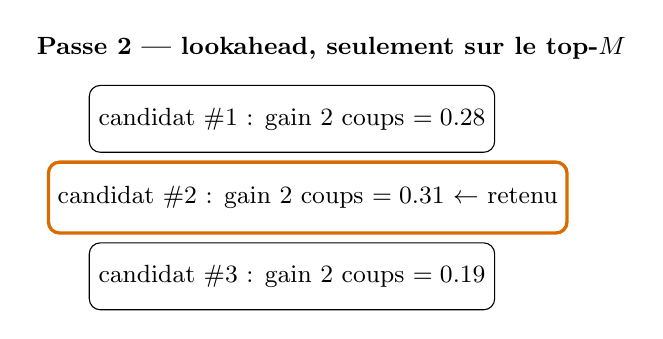
\begin{tikzpicture}
\node[font=\small\bfseries] at (2.6,1.9) {Passe 2 --- lookahead, seulement sur le top-$M$};
\node[draw, rounded corners, minimum width=4.2cm, minimum height=0.85cm, font=\small] at (2.1,1.0) {candidat \#1 : gain 2 coups $=0.28$};
\node[draw=orange!85!black, very thick, rounded corners, minimum width=4.6cm, minimum height=0.9cm, font=\small] at (2.3,0) {candidat \#2 : gain 2 coups $=0.31$ $\leftarrow$ retenu};
\node[draw, rounded corners, minimum width=4.2cm, minimum height=0.85cm, font=\small] at (2.1,-1.0) {candidat \#3 : gain 2 coups $=0.19$};
\end{tikzpicture}
\caption{Le classement glouton trie \emph{toutes} les features sans regarder plus
loin. Seuls les \code{LOOKAHEAD\_TOPM} meilleurs reçoivent la simulation d'un
second niveau de coupure (\code{LookaheadBuffers}) --- ce qui peut changer le
gagnant (le candidat \#2, moins bon au premier coup d'œil, l'emporte ici une fois
le deuxième niveau simulé).}
\label{fig:topm}
\end{figure}

\subsection{Choisir la feuille à couper : gain $\times$ masse}\label{sec:leafmass}

Une fois la meilleure coupure connue pour chaque feuille, laquelle couper en
premier ? Le code compare \code{leafBestGain * leafMass}, où \code{leafMass} est
la somme des poids des exemples de la feuille --- \textbf{pas} le gain seul.

\begin{figure}[h]
\centering
\begin{tikzpicture}[
  leafbox/.style={draw, rounded corners, minimum height=1.9cm, align=center, font=\small},
  arr/.style={-{Stealth[length=8pt]}, thick}
]
\node[leafbox, minimum width=2.6cm] (A) at (0,0) {feuille A\\gain $0.42$\\masse $0.05$\\[3pt]pondéré $=0.021$};
\node[leafbox, minimum width=2.6cm] (C) at (3.2,0) {feuille C\\gain $0.15$\\masse $0.10$\\[3pt]pondéré $=0.015$};
\node[leafbox, draw=orange!80!black, very thick, fill=orange!8, minimum width=7cm] (B) at (8.7,0)
  {\textbf{feuille B --- « fourre-tout »}\\
   gain local $0.08$ (le plus faible des trois)\\
   masse $0.61$ (61\% des exemples)\\[3pt]
   \bfseries pondéré $=0.049$ $\to$ maximum};
\node[leafbox, draw=orange!80!black, minimum width=2.2cm] (choix) at (13.6,0) {choisie\\$\checkmark$};
\draw[arr, orange!80!black] (B.east) -- (choix.west);
\end{tikzpicture}
\caption{Sans ce facteur de masse, une feuille géante mal triée (typique de
MNIST, où une immense feuille ``fourre-tout'' concentrait 53 à 89\% des
négatifs) n'était \emph{jamais} subdivisée : son gain \emph{local} semblait
toujours pire que celui de petites feuilles déjà quasi pures, alors qu'elle
concernait bien plus d'exemples au total. Ce correctif de pondération par la
masse est celui qui a fait progresser le plus l'accuracy sur MNIST.}
\label{fig:leafmass}
\end{figure}

% ======================================================
\section{Statuer sur chaque feuille finale}\label{sec:leaves}
% ======================================================

Une fois l'arbre figé ($K$ feuilles, ou moins si le lookahead ne trouve plus de
coupure utile), chaque feuille reçoit quatre étiquettes, calculées \textbf{une
seule fois} à partir des exemples pondérés qui y sont tombés.

\begin{description}
  \item[\code{frac1}] la proportion pondérée d'exemples $y{=}1$ :
    $\mathrm{frac1} = \mathrm{wPos}/\mathrm{wSum}$ sur les exemples de la feuille.
  \item[\code{leafIsPureZero}] vrai si $\mathrm{frac1} \le \code{noiseTol}$ ---
    la feuille est jugée presque toujours négative, même en tolérant un peu de
    bruit d'étiquette.
  \item[\code{leafMajorityVote}] $1$ si $\mathrm{frac1}\ge0.5$, sinon $0$ ---
    sert uniquement à la baseline diagnostique ``routeur seul'', jamais à la
    prédiction du système complet.
  \item[\code{leafWorstSkew}] on parcourt toutes les features \emph{encore
    libres} $f$ (non gelées par le chemin), on calcule leur proportion pondérée
    $q_f = P(x_f{=}1)$ dans la feuille, et on garde
    $\min_f \min(q_f, 1-q_f)$ --- la feature libre la plus déséquilibrée,
    c'est-à-dire la plus dangereuse pour l'apprentissage (section~\ref{sec:calib}).
\end{description}

\begin{exemple}
Pour la feuille C ($k{=}2$), features libres $\{1,3\}$ : si $x_1$ apparaît à
$q_1=0.47$ (presque équilibrée) et $x_3$ à $q_3=0.06$ (très déséquilibrée), alors
$\mathrm{leafWorstSkew} = \min(0.47,0.53,\,0.06,0.94) = 0.06$. C'est ce chiffre,
et non $0.47$, qui pilotera la calibration : le pire cas gouverne.
\end{exemple}

\begin{center}
\renewcommand{\arraystretch}{1.3}
\begin{tabular}{lccc}
\toprule
 & \textbf{feuille A} & \textbf{feuille B} & \textbf{feuille C} \\
\midrule
frac1 pondérée         & $0.03$ & $0.52$ & $0.18$ \\
\code{leafIsPureZero}  & vrai   & faux   & faux   \\
\code{leafMajorityVote}& $0$    & $1$    & $0$    \\
\code{leafWorstSkew}   & $0.31$ & $0.44$ & $0.06$ \\
\bottomrule
\end{tabular}
\end{center}

% ======================================================
\section{Calibrer $S$ et $\alpha$ contre les features déséquilibrées}\label{sec:calib}
% ======================================================

Un automate de Tsetlin standard suppose implicitement que ses deux issues
($x_i{=}0$ et $x_i{=}1$) sont à peu près équiprobables. Si une feature libre est
en réalité très déséquilibrée (ex. $q=0.06$, feuille C ci-dessus) --- sans être
totalement constante --- l'automate peut dériver vers $\Inc$ à tort, uniquement
parce qu'il voit rarement le cas contraire, pas parce que la feature est
informative. \code{calibrateParams(baseS, baseA, worstSkew)} réduit $S$ pour
neutraliser ce risque.

\subsection{D'où vient le seuil $B$}

On se place dans le pire cas : une feature libre de skew $q=\min(q_i,1-q_i)$,
totalement indépendante de $y$ (bruit pur), avec $y$ équilibré à 50/50 (garanti
par l'échantillonnage équilibré, section~\ref{sec:sampler}). Les probabilités de
transition de $v[i]$ deviennent (cf.\ le tableau à 4 cas, section~\ref{sec:update}) :
\[
  p^+_v = (1-q)\cdot\tfrac12\cdot S, \qquad
  p^-_v = (1-q)\cdot\tfrac12\cdot\alpha + q\cdot\tfrac12\cdot S.
\]
L'automate reste, à tort, poussé vers $\Inc$ tant que $p^+_v > p^-_v$, soit
$S/\alpha > (1-q)/(1-2q) =: B(q)$. $B(q)$ est donc le ratio $S/\alpha$
\textbf{au-delà duquel} une feature purement bruitée peut dériver vers $\Inc$.
\code{margin=4} impose une marge de sécurité : on veut rester \emph{sous}
$B(q)/4$, pas juste sous $B(q)$.

\begin{figure}[h]
\centering
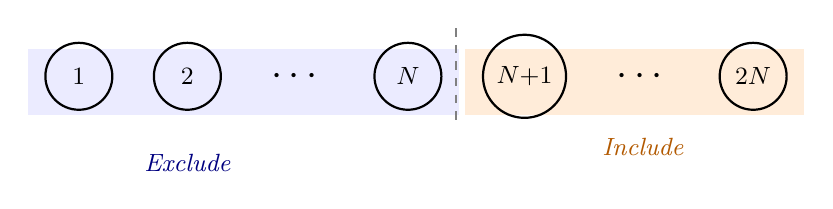
\begin{tikzpicture}[
  state/.style={circle, draw=black, thick, minimum size=0.85cm, font=\small},
  node distance=0.5cm
]
\node[state] (s1) {$1$};
\node[state, right=of s1] (s2) {$2$};
\node[right=0.5cm of s2, font=\Large] (d1) {$\cdots$};
\node[state, right=0.5cm of d1] (sN) {$N$};
\node[state, right=of sN] (sN1) {\small$N{+}1$};
\node[right=0.5cm of sN1, font=\Large] (d2) {$\cdots$};
\node[state, right=0.5cm of d2] (s2N) {$2N$};
\begin{scope}[on background layer]
  \fill[blue!8]  ([xshift=-6pt,yshift=-14pt]s1.west)  rectangle ([xshift=6pt,yshift=10pt]sN.east);
  \fill[orange!15] ([xshift=-6pt,yshift=-14pt]sN1.west) rectangle ([xshift=6pt,yshift=10pt]s2N.east);
\end{scope}
\node[below=12pt of s2, font=\small\itshape, text=blue!50!black] {Exclude};
\node[below=12pt of d2, font=\small\itshape, text=orange!70!black] {Include};
\draw[dashed, gray] ($(sN.north east)+(0.3,0.3)$) -- ($(sN.south east)+(0.3,-0.25)$);
\end{tikzpicture}
\caption{L'état d'un automate se lit sur une seule droite : au-dessus de $N$,
\Inc ; à $N$ ou en-dessous, \Exc.}
\label{fig:automate-line}
\end{figure}

\begin{figure}[h]
\centering
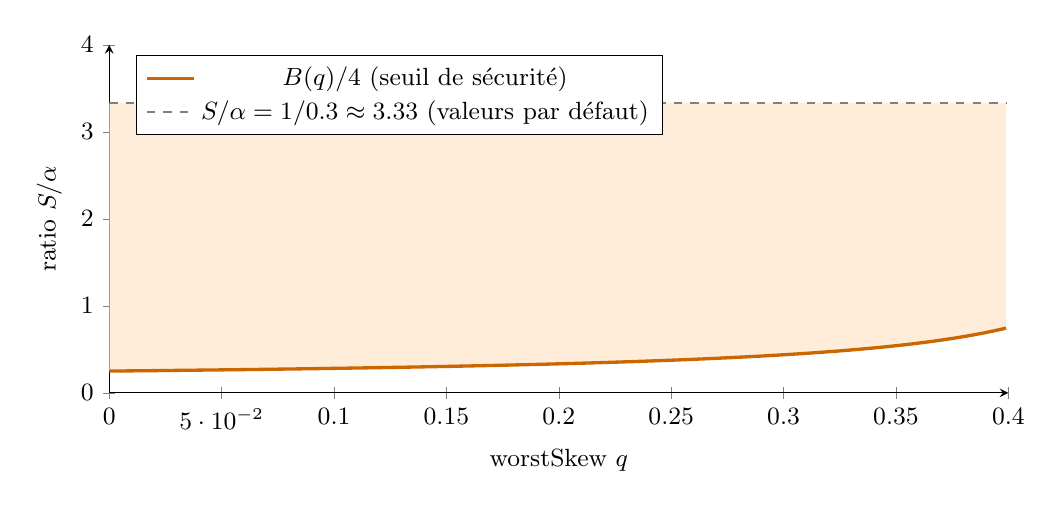
\begin{tikzpicture}
\begin{axis}[
  width=13cm, height=6cm,
  xlabel={worstSkew $q$}, ylabel={ratio $S/\alpha$},
  xmin=0, xmax=0.4, ymin=0, ymax=4,
  domain=0:0.399, samples=80,
  legend pos=north west, legend style={font=\small},
  axis lines=left, tick label style={font=\small}, label style={font=\small}
]
\addplot[name path=B, orange!80!black, very thick] {(1-x)/(1-2*x)/4};
\addlegendentry{$B(q)/4$ (seuil de sécurité)}
\addplot[name path=D, gray, dashed, thick] {3.333};
\addlegendentry{$S/\alpha=1/0.3\approx 3.33$ (valeurs par défaut)}
\addplot[orange!15] fill between[of=B and D];
\end{axis}
\end{tikzpicture}
\caption{Pour $S{=}1,\alpha{=}0.3$ (défaut), le ratio $3.33$ reste toujours
au-dessus de $B(q)/4$ tant que $q<0.40$ (zone orange) : la calibration
\textbf{s'active systématiquement} pour toute feature libre avec
$\mathrm{leafWorstSkew}<0.40$. Elle ne garde les valeurs par défaut que si la
feuille n'a plus de feature libre vraiment déséquilibrée ($q\ge0.40$).}
\label{fig:calib-curve}
\end{figure}

\noindent Concrètement, quand $q<0.40$ : \code{calibrateParams} fixe $\alpha{=}1$
et $S = (B(q)/4)\cdot\alpha$, ce qui ramène exactement le ratio $S/\alpha$ à la
limite de sécurité $B(q)/4$ --- ni plus prudent que nécessaire, ni moins.

% ======================================================
\section{Geler les features du routeur, verrouiller les feuilles PureZero}\label{sec:gel}
% ======================================================

Une clause ne doit \textbf{pas} réapprendre ce que le routeur a déjà décidé : à
l'intérieur d'une feuille donnée, une feature gelée est \emph{constante} (par
construction, tous les exemples de la feuille C ont $x_0{=}1$). Un automate
confronté à une feature constante ne voit jamais qu'une seule des deux lignes du
tableau à 4 cas : il dérive dans une seule direction, sans aucune force
contraire pour l'arrêter --- ce n'est pas un problème d'apprentissage lent, c'est
une dérive garantie. La solution : ne pas apprendre du tout sur ces features,
et fixer leurs deux automates une fois pour toutes à la construction du réseau.

\subsection{Cas standard : exclure les deux littéraux}

Pour une feature gelée $i$, si la feuille n'est \textbf{pas} PureZero, le code fixe
simplement $v[i].\mathrm{state}=1$ et $\vbar[i].\mathrm{state}=1$ : les deux
littéraux sont \Exc, la feature \textbf{n'apparaît plus du tout} dans la clause
(cadran ``absent de la clause'' de la figure~\ref{fig:config-rappel}). C'est le
cas de $\{0,2\}$ pour la feuille C dans l'exemple fil rouge (section~\ref{sec:pipeline}).

\subsection{Cas PureZero : verrouiller la sortie à 0}

Pour la feuille A (PureZero, $\mathrm{frac1}=0.03$), le code exploite en plus ce
qu'on sait déjà : cette feuille est presque toujours négative. Plutôt que de
laisser la clause l'apprendre (ce qui gaspillerait un littéral et prendrait du
temps), on \textbf{câble en dur} un unique littéral garanti faux.

\begin{exemple}
En feuille A, $x_0$ est fixée à $0$. Puisque $\mathrm{leafFixedValue}=0$, le code
force $v[0].\mathrm{state}=2N$ (\Inc) et $\vbar[0].\mathrm{state}=1$ (\Exc). Le
littéral inclus est donc ``$x_0$'' --- or $x_0\equiv0$ dans cette feuille, donc ce
littéral est \textbf{toujours violé}. Dès qu'un littéral inclus est violé, la
clause entière est violée (section~\ref{sec:update-sortie}) : \textbf{output$(x)=0$
pour tout $x$ de cette feuille}, sans qu'aucun automate n'ait eu besoin
d'apprendre quoi que ce soit.
\end{exemple}

\begin{figure}[h]
\centering
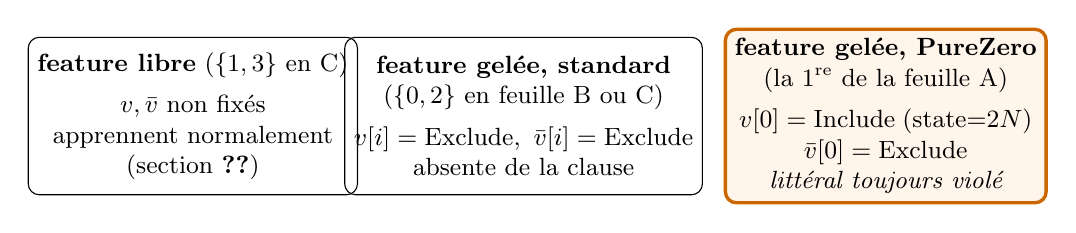
\begin{tikzpicture}[
  cell/.style={draw, rounded corners, minimum width=3.4cm, minimum height=2cm, align=center, font=\small},
]
\node[cell] (free) at (0,0)
  {\textbf{feature libre} ($\{1,3\}$ en C)\\[4pt]$v,\vbar$ non fixés\\apprennent normalement\\(section~\ref{sec:update})};
\node[cell] (froz) at (4.2,0)
  {\textbf{feature gelée, standard}\\($\{0,2\}$ en feuille B ou C)\\[4pt]$v[i]=\Exc,\ \vbar[i]=\Exc$\\absente de la clause};
\node[cell, draw=orange!80!black, very thick, fill=orange!8] (forced) at (8.8,0)
  {\textbf{feature gelée, PureZero}\\(la 1\textsuperscript{re} de la feuille A)\\[4pt]
   $v[0]=\Inc\;(\mathrm{state}{=}2N)$\\$\vbar[0]=\Exc$\\\itshape littéral toujours violé};
\end{tikzpicture}
\caption{Les trois traitements possibles d'une feature à la construction du
réseau. Un seul littéral forcé par feuille suffit : \code{score()} retourne
``violé'' dès que \emph{n'importe quel} littéral inclus est faux
(section~\ref{sec:update-sortie}).}
\label{fig:freeze}
\end{figure}

% ======================================================
\section{Mettre à jour une clause : la règle à 4 cas, masquée}\label{sec:update}
% ======================================================

En dehors des features gelées, une clause apprend exactement la règle à 4 cas
démontrée dans \emph{convergence\_sans\_bruit.tex} --- \code{updateMasked} se
contente de sauter les features où \code{active[i]=false}.

\begin{center}
\renewcommand{\arraystretch}{1.4}
\begin{tabular}{ccll}
\toprule
$x[i]$ & $y$ & Action sur $v[i]$ (littéral $x_i$) & Action sur $\vbar[i]$ (littéral $\neg x_i$) \\
\midrule
0 & 0 & \code{towardInclude}$(S)$   & \code{towardExclude}$(S)$ \\
0 & 1 & \code{towardExclude}$(\alpha)$ & rien \\
1 & 0 & \code{towardExclude}$(S)$   & \code{towardInclude}$(S)$ \\
1 & 1 & rien                      & \code{towardExclude}$(\alpha)$ \\
\bottomrule
\end{tabular}
\end{center}

\begin{exemple}
Reprenons $x=(1,1,1,0)$ routé en feuille C, avec $y=1$ (vrai label de cet
exemple). Seules les features libres $\{1,3\}$ sont mises à jour :
\begin{itemize}
  \item $i=1$ : $x_1{=}1,\,y{=}1 \Rightarrow$ rien sur $v[1]$, et
        $\vbar[1]$ fait \code{towardExclude}$(\alpha)$ ;
  \item $i=3$ : $x_3{=}0,\,y{=}1 \Rightarrow$ $v[3]$ fait
        \code{towardExclude}$(\alpha)$, rien sur $\vbar[3]$.
\end{itemize}
$v[0],\vbar[0],v[2],\vbar[2]$ (gelées) ne bougent pas.
\end{exemple}

\subsection{Comment la clause répond ensuite : les trois cas de \code{score()}}\label{sec:update-sortie}

\begin{center}
\renewcommand{\arraystretch}{1.3}
\begin{tabular}{clll}
\toprule
Cas & Condition & \code{score()} & Sens \\
\midrule
1 & aucun littéral inclus & $0$ & clause vide, neutre \\
2 & $\ge1$ littéral inclus violé & $-\mathrm{violated}$ & confiance que ce n'est \textbf{pas} cette classe \\
3 & tous les littéraux inclus satisfaits & $+\mathrm{satisfied}$ & confiance que c'est cette classe \\
\bottomrule
\end{tabular}
\end{center}

% ======================================================
\section{Entraîner : tirage équilibré, \code{total} mises à jour}\label{sec:sampler}
% ======================================================

\code{WeightedSampler} garantit que chaque mise à jour voit la classe $0$ et la
classe $1$ avec une probabilité $50/50$ --- même si le dataset réel est
déséquilibré --- tout en respectant, \emph{à l'intérieur} de chaque classe, les
poids du boosting (les exemples que le round précédent a mal classés sont tirés
plus souvent).

\begin{figure}[h]
\centering
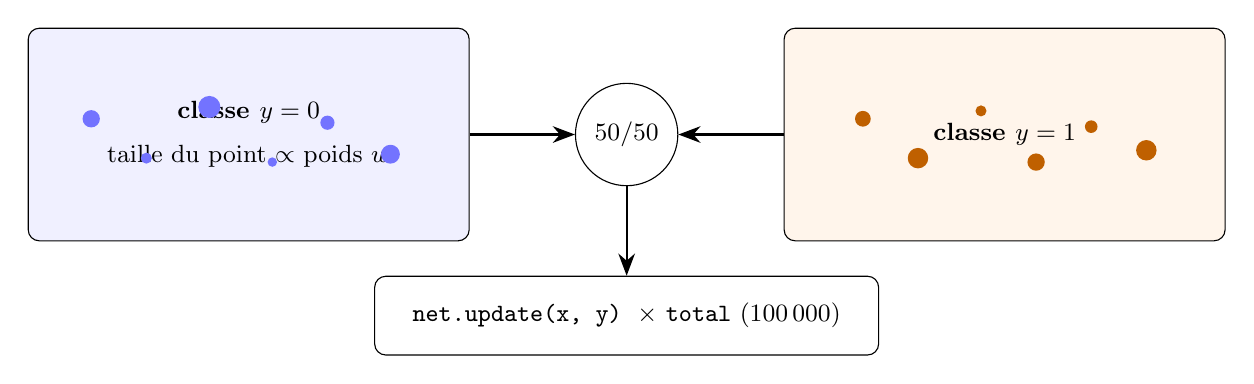
\begin{tikzpicture}
\node[draw, rounded corners, minimum width=5.6cm, minimum height=2.7cm, fill=blue!6, align=center] (c0) at (0,0)
     {\small\bfseries classe $y=0$\\[0.4em]\small taille du point $\propto$ poids $w$};
\foreach \x/\y/\r in {-2.0/0.2/0.11, -1.3/-0.3/0.07, -0.5/0.35/0.14, 0.3/-0.35/0.06, 1.0/0.15/0.09, 1.8/-0.25/0.12}
  \fill[blue!55] (\x,\y) circle (\r);

\node[draw, rounded corners, minimum width=5.6cm, minimum height=2.7cm, fill=orange!8, align=center] (c1) at (9.6,0)
     {\small\bfseries classe $y=1$};
\foreach \x/\y/\r in {7.8/0.2/0.10, 8.5/-0.3/0.13, 9.3/0.3/0.07, 10.0/-0.35/0.11, 10.7/0.1/0.08, 11.4/-0.2/0.13}
  \fill[orange!75!black] (\x,\y) circle (\r);

\node[draw, circle, minimum size=1.3cm, fill=white] (coin) at (4.8,0) {\small 50/50};
\draw[-{Stealth[length=8pt]}, thick] (c0.east) -- (coin.west);
\draw[-{Stealth[length=8pt]}, thick] (c1.west) -- (coin.east);

\node[draw, rounded corners, minimum width=6.4cm, minimum height=1cm, font=\small] (upd) at (4.8,-2.3)
     {\code{net.update(x, y)}\; $\times$ \code{total} (100\,000)};
\draw[-{Stealth[length=8pt]}, thick] (coin.south) -- (upd.north);
\end{tikzpicture}
\caption{À chaque tirage : pile ou face 50/50 pour choisir la classe, puis
tirage pondéré (\code{discrete\_distribution}) par poids $w$ à l'intérieur de
cette classe. C'est ce rééquilibrage systématique qui rend valide l'hypothèse
``$y$ à 50/50'' utilisée dans la dérivation de \code{calibrateParams}
(section~\ref{sec:calib}).}
\label{fig:sampler}
\end{figure}

% ======================================================
\section{Mesurer l'erreur, pondérer (AdaBoost)}
% ======================================================

Une fois les \code{total} mises à jour terminées, le réseau du round est évalué
sur \textbf{tout} l'ensemble d'entraînement (pas seulement le lot de découverte),
pondéré par les poids courants $w$ :
\[
  \mathrm{err} = \frac{\displaystyle\sum_{i \text{ mal classé}} w_i}{\displaystyle\sum_i w_i}
  \ \in\ [10^{-6},\,0.999],
  \qquad
  \alpha = \frac12\ln\!\left(\frac{1-\mathrm{err}}{\mathrm{err}}\right).
\]
$\alpha$ est grand si $\mathrm{err}$ est petit (le round est fiable, on lui donne
une forte voix au moment de combiner, section~\ref{sec:combine}) et proche de $0$
si $\mathrm{err}\approx0.5$ (le round n'a fait guère mieux que le hasard).
Ensuite, chaque poids est mis à jour puis renormalisé :
\[
  w_i \mathrel{*}= \begin{cases} e^{\alpha} & \text{si } i \text{ mal classé} \\ e^{-\alpha} & \text{sinon}\end{cases}
  \qquad\text{puis}\qquad w_i \mathrel{/}= \textstyle\sum_i w_i.
\]

\begin{figure}[h]
\centering
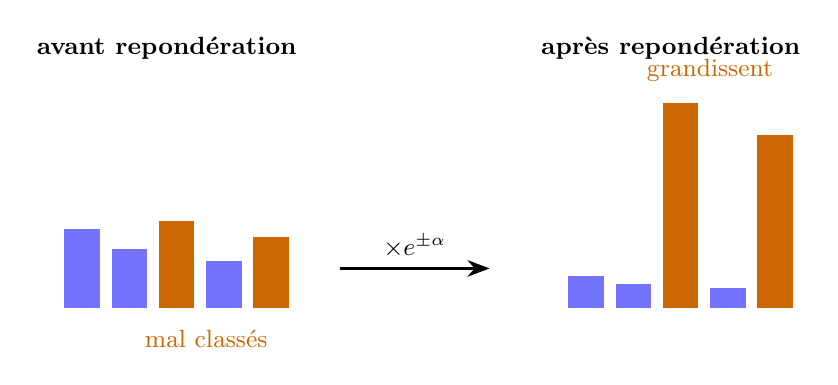
\begin{tikzpicture}
\node[font=\small\bfseries] at (1.3,3.3) {avant repondération};
\foreach \x/\h/\c in {0/1.0/blue!55, 0.6/0.75/blue!55, 1.2/1.1/orange!80!black, 1.8/0.6/blue!55, 2.4/0.9/orange!80!black}
  \draw[fill=\c, draw=none] (\x,0) rectangle (\x+0.45,\h);
\node[font=\small, orange!80!black] at (1.8,-0.4) {mal classés};

\draw[-{Stealth[length=8pt]}, thick] (3.5,0.5) -- (5.4,0.5) node[midway, above, font=\small] {$\times e^{\pm\alpha}$};

\begin{scope}[xshift=6.4cm]
\node[font=\small\bfseries] at (1.3,3.3) {après repondération};
\foreach \x/\h/\c in {0/0.4/blue!55, 0.6/0.3/blue!55, 1.2/2.6/orange!80!black, 1.8/0.25/blue!55, 2.4/2.2/orange!80!black}
  \draw[fill=\c, draw=none] (\x,0) rectangle (\x+0.45,\h);
\node[font=\small, orange!80!black, above] at (1.8,2.75) {grandissent};
\end{scope}
\end{tikzpicture}
\caption{Les exemples mal classés voient leur poids croître, les bien classés
décroître (puis tout est renormalisé). Le \emph{prochain} \code{discoverBatch}
(trié par $w$, section~\ref{sec:router}) sera donc dominé par les exemples
encore mal classés : le round suivant est forcé de router et d'apprendre
spécifiquement là où le round précédent a échoué.}
\label{fig:adaboost}
\end{figure}

% ======================================================
\section{Combiner les $M$ réseaux et décider}\label{sec:combine}
% ======================================================

Après les $M$ rounds, chaque réseau vote avec son \code{score()}, normalisé par
le nombre de littéraux de la clause utilisée ($\mathrm{normalizedScore} =
\mathrm{score}/n_{\mathrm{lit}}$, pour rendre les votes comparables entre
clauses de tailles différentes), pondéré par la confiance $\alpha_m$ que le
boosting lui a accordée :
\[
  \mathrm{score}(x) = \sum_{m=1}^{M} \alpha_m \cdot \mathrm{normalizedScore}_m(x),
  \qquad
  \hat y = \begin{cases}1 & \text{si } \mathrm{score}(x) > 0\\ 0 & \text{sinon.}\end{cases}
\]

\begin{figure}[h]
\centering
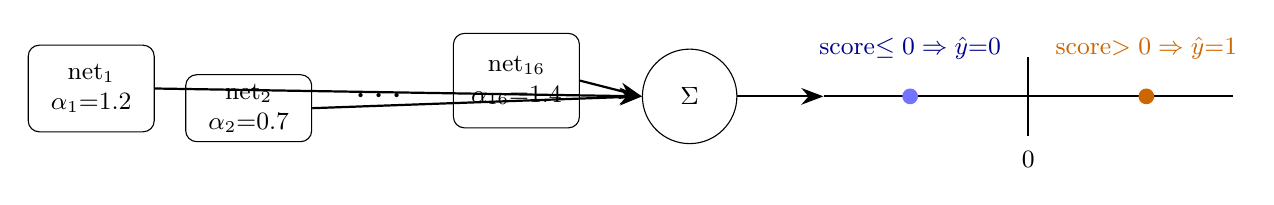
\begin{tikzpicture}
\node[draw, rounded corners, minimum width=1.6cm, minimum height=1.1cm, font=\small, align=center] (n1) at (0,0.4) {net$_1$\\$\alpha_1{=}1.2$};
\node[draw, rounded corners, minimum width=1.6cm, minimum height=0.8cm, font=\small, align=center] (n2) at (2.0,0.15) {net$_2$\\$\alpha_2{=}0.7$};
\node[font=\Large] at (3.7,0.3) {$\cdots$};
\node[draw, rounded corners, minimum width=1.6cm, minimum height=1.2cm, font=\small, align=center] (nM) at (5.4,0.5) {net$_{16}$\\$\alpha_{16}{=}1.4$};

\node[draw, circle, minimum size=1.2cm, font=\small] (sum) at (7.6,0.3) {$\Sigma$};
\draw[-{Stealth[length=8pt]}, thick] (n1.east) -- (sum.west);
\draw[-{Stealth[length=8pt]}, thick] (n2.east) -- (sum.west);
\draw[-{Stealth[length=8pt]}, thick] (nM.east) -- (sum.west);

\draw[-{Stealth[length=8pt]}, thick] (sum.east) -- (9.3,0.3);
\draw[thick] (9.3,0.3) -- (14.5,0.3);
\draw[thick] (11.9,-0.2) -- (11.9,0.8);
\node[font=\small] at (11.9,-0.5) {0};
\fill[blue!55] (10.4,0.3) circle (0.1);
\node[font=\small, blue!55!black, above] at (10.4,0.65) {score$\le0\Rightarrow\hat y{=}0$};
\fill[orange!80!black] (13.4,0.3) circle (0.1);
\node[font=\small, orange!80!black, above] at (13.4,0.65) {score$>0\Rightarrow\hat y{=}1$};
\end{tikzpicture}
\caption{Vote pondéré final : un round fiable (grand $\alpha$) pèse fort, un
round peu fiable pèse peu --- le mécanisme AdaBoost standard, appliqué ici à des
réseaux routeur+clauses plutôt qu'à des souches de décision classiques.}
\label{fig:combine}
\end{figure}

\begin{note}
En parallèle de $\mathrm{score}(x)$, chaque fichier de validation calcule aussi
une \emph{baseline} $\sum_m \alpha_m\,(\mathrm{leafMajorityPurity}_m[\mathrm{leaf}]-0.5)$
--- le même vote pondéré, mais en remplaçant la clause par la simple pureté de
la feuille où l'exemple atterrit. Comparer les deux accuracies (ex. XOR :
$100.0\%$ avec clauses contre $50.1\%$ sans) est la preuve empirique que ce sont
bien les \textbf{clauses}, et non le seul routeur, qui portent la prédiction.
\end{note}

% ======================================================
\section{Où tout ceci s'inscrit : le round complet}\label{sec:pipeline}
% ======================================================

Les sections précédentes détaillent \emph{une passe d'inférence} (comment un
réseau déjà construit répond à un exemple) et les mécanismes de construction
(routeur, gel, calibration). Ensemble, ils forment un round de
\code{trainBoostedClass}, répété $M$ fois :

\begin{figure}[h]
\centering
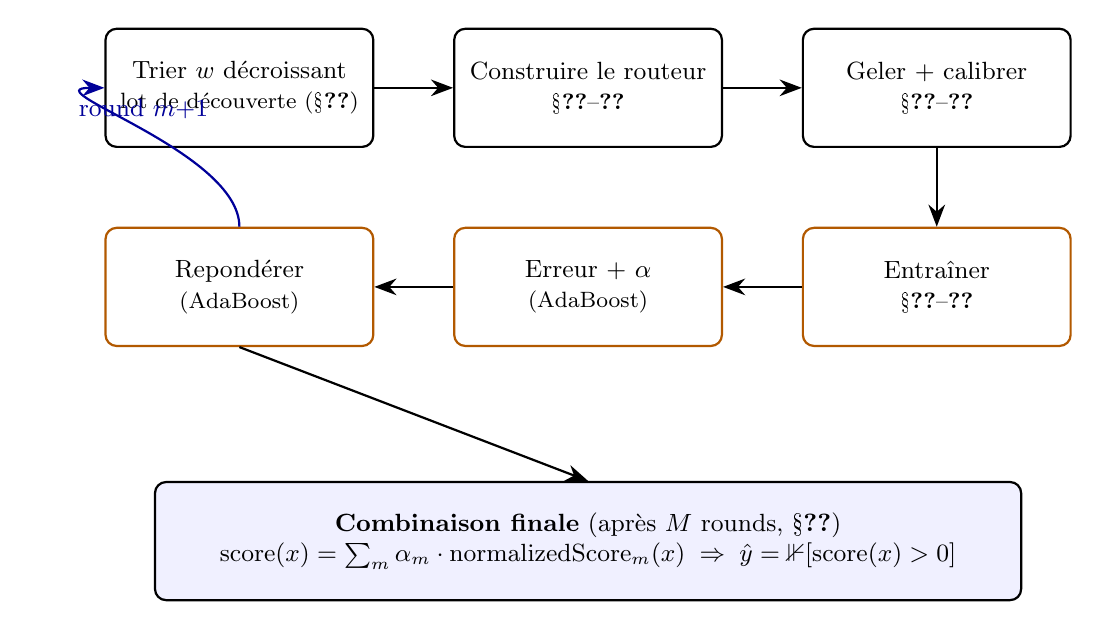
\begin{tikzpicture}[
  box/.style={draw, rounded corners, thick, minimum width=3.4cm, minimum height=1.5cm,
              align=center, font=\small},
  boxw/.style={box, draw=orange!70!black},
  arr/.style={-{Stealth[length=8pt]}, thick},
  node distance=1cm and 1cm
]
\node[box] (b1) {Trier $w$ décroissant\\\footnotesize lot de découverte (\S\ref{sec:router})};
\node[box, right=of b1] (b2) {Construire le routeur\\\footnotesize \S\ref{sec:router}--\ref{sec:leaves}};
\node[box, right=of b2] (b3) {Geler + calibrer\\\footnotesize \S\ref{sec:calib}--\ref{sec:gel}};

\node[boxw, below=of b3] (b4) {Entraîner\\\footnotesize \S\ref{sec:sampler}--\ref{sec:update}};
\node[boxw, left=of b4] (b5) {Erreur $+$ $\alpha$\\\footnotesize (AdaBoost)};
\node[boxw, left=of b5] (b6) {Repondérer\\\footnotesize (AdaBoost)};

\draw[arr] (b1) -- (b2);
\draw[arr] (b2) -- (b3);
\draw[arr] (b3) -- (b4);
\draw[arr] (b4) -- (b5);
\draw[arr] (b5) -- (b6);
\draw[arr, blue!60!black] (b6.north) to[out=90,in=180] node[above,font=\small,text=blue!60!black]{round $m{+}1$} (b1.west);

\node[box, below=1.7cm of b5, minimum width=11cm, fill=blue!6] (final)
  {\textbf{Combinaison finale} (après $M$ rounds, \S\ref{sec:combine})\\
   $\mathrm{score}(x)=\sum_m \alpha_m\cdot\mathrm{normalizedScore}_m(x)
   \;\Rightarrow\;\hat y = \mathbb{1}[\mathrm{score}(x)>0]$};
\draw[arr] (b6.south) -- (final.north);
\end{tikzpicture}
\caption{Le round de boosting complet. Ce schéma est identique pour les quatre
datasets validés --- seuls $n$, $K$, $M$ et \code{noiseTol} changent d'un
fichier à l'autre.}
\label{fig:overview}
\end{figure}

\vfill
\hrule
\vspace{0.4em}
\noindent\footnotesize
\textbf{Portée} : \code{trainBoostedClass} $\cdot$ \code{buildWeightedRouterTree}
$\cdot$ \code{calibrateParams} $\cdot$ \code{MultiClauseNetwork} --- tous dans
\texttt{tsetlin\_engine.h}. Appliqué identiquement à Iris, Digits, XOR, MNIST.

\end{document}
